\documentclass[11pt]{article}
\usepackage[review]{acl}
\usepackage{times}
\usepackage{latexsym}
\usepackage[T1]{fontenc}
\usepackage[utf8]{inputenc}
\usepackage{microtype}
\usepackage{graphicx}
\usepackage{booktabs}
\usepackage{amsmath}

% Every number comes from scripts/paper_tables.py. A missing key stops the build instead of printing nothing.
\expandafter\def\csname v@intern.blank\endcsname{54.3}
\expandafter\def\csname v@intern.blankref\endcsname{100.0}
\expandafter\def\csname v@intern.box\endcsname{85.0}
\expandafter\def\csname v@intern.cf\endcsname{81.1}
\expandafter\def\csname v@intern.n\endcsname{127}
\expandafter\def\csname v@intern.null\endcsname{+0.0}
\expandafter\def\csname v@intern.s100.au\endcsname{0.73}
\expandafter\def\csname v@intern.s100.auc\endcsname{0.57}
\expandafter\def\csname v@intern.s100.aucin\endcsname{0.60}
\expandafter\def\csname v@intern.s100.confmean\endcsname{100.9}
\expandafter\def\csname v@intern.s100.confout\endcsname{1}
\expandafter\def\csname v@intern.s100.disc\endcsname{+40.0 [+0.0, +100.0]}
\expandafter\def\csname v@intern.s100.hijack\endcsname{18.1}
\expandafter\def\csname v@intern.s100.hijacktarget\endcsname{63.8}
\expandafter\def\csname v@intern.s100.orig\endcsname{80.3}
\expandafter\def\csname v@intern.s100.prog\endcsname{-2.4 [-11.0, +6.3]}
\expandafter\def\csname v@intern.s100.refgap\endcsname{+20.1 [+4.4, +38.3]}
\expandafter\def\csname v@intern.s100.refrate\endcsname{7.9}
\expandafter\def\csname v@intern.s100.task\endcsname{+5.5 [-0.8, +12.6]}
\expandafter\def\csname v@intern.s30.G\endcsname{76.4}
\expandafter\def\csname v@intern.s30.L\endcsname{44.9}
\expandafter\def\csname v@intern.s30.LG\endcsname{88.2}
\expandafter\def\csname v@intern.s30.O\endcsname{0.0}
\expandafter\def\csname v@intern.s30.au\endcsname{0.79}
\expandafter\def\csname v@intern.s30.auc\endcsname{0.47}
\expandafter\def\csname v@intern.s30.aucin\endcsname{0.48}
\expandafter\def\csname v@intern.s30.base\endcsname{63.0}
\expandafter\def\csname v@intern.s30.boxBlur\endcsname{-18.1 [-26.8, -9.4]}
\expandafter\def\csname v@intern.s30.boxSharp\endcsname{+11.8 [+4.7, +19.7]}
\expandafter\def\csname v@intern.s30.confmean\endcsname{99.2}
\expandafter\def\csname v@intern.s30.confout\endcsname{1}
\expandafter\def\csname v@intern.s30.disc\endcsname{+82.8 [+70.0, +93.8]}
\expandafter\def\csname v@intern.s30.inter\endcsname{+29.9 [+20.5, +39.4]}
\expandafter\def\csname v@intern.s30.orig\endcsname{62.2}
\expandafter\def\csname v@intern.s30.phiG\endcsname{+28.3 [+22.4, +34.6]}
\expandafter\def\csname v@intern.s30.phiL\endcsname{-3.1 [-9.4, +3.5]}
\expandafter\def\csname v@intern.s30.prog\endcsname{-5.5 [-14.2, +3.1]}
\expandafter\def\csname v@intern.s30.pull\endcsname{+0.0 [+0.0, +0.0]}
\expandafter\def\csname v@intern.s30.refgap\endcsname{+13.2 [+0.6, +26.3]}
\expandafter\def\csname v@intern.s30.refrate\endcsname{12.6}
\expandafter\def\csname v@intern.s30.task\endcsname{+3.1 [-3.9, +10.2]}
\expandafter\def\csname v@intern.s30.upscale\endcsname{+0.8 [+0.0, +2.4]}
\expandafter\def\csname v@intern.s40.G\endcsname{79.5}
\expandafter\def\csname v@intern.s40.L\endcsname{76.4}
\expandafter\def\csname v@intern.s40.LG\endcsname{90.6}
\expandafter\def\csname v@intern.s40.O\endcsname{0.0}
\expandafter\def\csname v@intern.s40.au\endcsname{0.76}
\expandafter\def\csname v@intern.s40.auc\endcsname{0.45}
\expandafter\def\csname v@intern.s40.aucin\endcsname{0.47}
\expandafter\def\csname v@intern.s40.base\endcsname{80.3}
\expandafter\def\csname v@intern.s40.boxBlur\endcsname{-3.9 [-11.8, +4.0]}
\expandafter\def\csname v@intern.s40.boxSharp\endcsname{+11.0 [+4.7, +18.1]}
\expandafter\def\csname v@intern.s40.confmean\endcsname{100.3}
\expandafter\def\csname v@intern.s40.confout\endcsname{1}
\expandafter\def\csname v@intern.s40.disc\endcsname{+55.6 [+25.0, +85.7]}
\expandafter\def\csname v@intern.s40.hijack\endcsname{14.2}
\expandafter\def\csname v@intern.s40.hijacktarget\endcsname{59.8}
\expandafter\def\csname v@intern.s40.inter\endcsname{+15.0 [+7.9, +22.0]}
\expandafter\def\csname v@intern.s40.orig\endcsname{80.3}
\expandafter\def\csname v@intern.s40.phiG\endcsname{+6.7 [+2.4, +11.0]}
\expandafter\def\csname v@intern.s40.phiL\endcsname{+3.5 [-2.8, +9.8]}
\expandafter\def\csname v@intern.s40.prog\endcsname{-1.6 [-10.2, +7.1]}
\expandafter\def\csname v@intern.s40.pull\endcsname{+0.0 [+0.0, +0.0]}
\expandafter\def\csname v@intern.s40.refgap\endcsname{+23.1 [+5.0, +42.0]}
\expandafter\def\csname v@intern.s40.refrate\endcsname{9.4}
\expandafter\def\csname v@intern.s40.task\endcsname{+7.9 [+0.8, +15.7]}
\expandafter\def\csname v@intern.s40.upscale\endcsname{+0.0 [-2.4, +2.4]}
\expandafter\def\csname v@intern.s50.G\endcsname{81.1}
\expandafter\def\csname v@intern.s50.L\endcsname{84.3}
\expandafter\def\csname v@intern.s50.LG\endcsname{90.6}
\expandafter\def\csname v@intern.s50.O\endcsname{0.0}
\expandafter\def\csname v@intern.s50.au\endcsname{0.76}
\expandafter\def\csname v@intern.s50.auc\endcsname{0.49}
\expandafter\def\csname v@intern.s50.aucin\endcsname{0.51}
\expandafter\def\csname v@intern.s50.base\endcsname{82.7}
\expandafter\def\csname v@intern.s50.boxBlur\endcsname{+1.6 [-6.3, +9.4]}
\expandafter\def\csname v@intern.s50.boxSharp\endcsname{+9.4 [+3.1, +16.5]}
\expandafter\def\csname v@intern.s50.confmean\endcsname{100.0}
\expandafter\def\csname v@intern.s50.confout\endcsname{1}
\expandafter\def\csname v@intern.s50.disc\endcsname{+83.3 [+60.0, +100.0]}
\expandafter\def\csname v@intern.s50.inter\endcsname{+7.9 [+3.1, +13.4]}
\expandafter\def\csname v@intern.s50.orig\endcsname{81.9}
\expandafter\def\csname v@intern.s50.phiG\endcsname{+2.4 [+0.4, +4.7]}
\expandafter\def\csname v@intern.s50.phiL\endcsname{+5.5 [-1.2, +12.2]}
\expandafter\def\csname v@intern.s50.prog\endcsname{-3.9 [-11.8, +3.9]}
\expandafter\def\csname v@intern.s50.pull\endcsname{+0.0 [+0.0, +0.0]}
\expandafter\def\csname v@intern.s50.refgap\endcsname{+30.9 [+10.7, +51.4]}
\expandafter\def\csname v@intern.s50.refrate\endcsname{9.4}
\expandafter\def\csname v@intern.s50.task\endcsname{+7.1 [+1.6, +13.4]}
\expandafter\def\csname v@intern.s50.upscale\endcsname{+0.8 [+0.0, +2.4]}
\expandafter\def\csname v@seven.attr.crit\endcsname{+37.7 [+31.7, +44.3]}
\expandafter\def\csname v@seven.attr.dshare\endcsname{+39.7 [+33.0, +46.3]}
\expandafter\def\csname v@seven.attr.n\endcsname{360}
\expandafter\def\csname v@seven.attr.s100.share\endcsname{10\%}
\expandafter\def\csname v@seven.attr.s30.share\endcsname{50\%}
\expandafter\def\csname v@seven.blank\endcsname{34.4}
\expandafter\def\csname v@seven.blankref\endcsname{100.0}
\expandafter\def\csname v@seven.box\endcsname{91.3}
\expandafter\def\csname v@seven.cf\endcsname{86.7}
\expandafter\def\csname v@seven.n\endcsname{218}
\expandafter\def\csname v@seven.null\endcsname{-1.4}
\expandafter\def\csname v@seven.s100.au\endcsname{0.80}
\expandafter\def\csname v@seven.s100.auc\endcsname{0.50}
\expandafter\def\csname v@seven.s100.aucin\endcsname{0.50}
\expandafter\def\csname v@seven.s100.confmean\endcsname{100.0}
\expandafter\def\csname v@seven.s100.confout\endcsname{0}
\expandafter\def\csname v@seven.s100.disc\endcsname{+55.6 [+31.2, +81.2]}
\expandafter\def\csname v@seven.s100.hijack\endcsname{1.4}
\expandafter\def\csname v@seven.s100.hijacktarget\endcsname{80.7}
\expandafter\def\csname v@seven.s100.orig\endcsname{88.1}
\expandafter\def\csname v@seven.s100.prog\endcsname{+0.5 [-5.0, +6.0]}
\expandafter\def\csname v@seven.s100.refgap\endcsname{+16.1 [+1.8, +32.8]}
\expandafter\def\csname v@seven.s100.refrate\endcsname{5.0}
\expandafter\def\csname v@seven.s100.task\endcsname{+0.0 [-2.3, +2.3]}
\expandafter\def\csname v@seven.s30.G\endcsname{85.3}
\expandafter\def\csname v@seven.s30.L\endcsname{65.1}
\expandafter\def\csname v@seven.s30.LG\endcsname{92.2}
\expandafter\def\csname v@seven.s30.O\endcsname{0.9}
\expandafter\def\csname v@seven.s30.au\endcsname{0.87}
\expandafter\def\csname v@seven.s30.auc\endcsname{0.51}
\expandafter\def\csname v@seven.s30.aucin\endcsname{0.51}
\expandafter\def\csname v@seven.s30.base\endcsname{68.8}
\expandafter\def\csname v@seven.s30.boxBlur\endcsname{-3.7 [-11.5, +4.1]}
\expandafter\def\csname v@seven.s30.boxSharp\endcsname{+6.9 [+2.3, +11.9]}
\expandafter\def\csname v@seven.s30.confmean\endcsname{98.6}
\expandafter\def\csname v@seven.s30.confout\endcsname{0}
\expandafter\def\csname v@seven.s30.disc\endcsname{+77.7 [+68.8, +85.9]}
\expandafter\def\csname v@seven.s30.inter\endcsname{+10.6 [+3.2, +17.9]}
\expandafter\def\csname v@seven.s30.orig\endcsname{38.5}
\expandafter\def\csname v@seven.s30.phiG\endcsname{+21.8 [+17.2, +26.6]}
\expandafter\def\csname v@seven.s30.phiL\endcsname{+1.6 [-3.9, +7.1]}
\expandafter\def\csname v@seven.s30.prog\endcsname{-0.9 [-6.9, +5.0]}
\expandafter\def\csname v@seven.s30.pull\endcsname{+0.9 [+0.0, +2.3]}
\expandafter\def\csname v@seven.s30.refgap\endcsname{+11.2 [+6.3, +16.9]}
\expandafter\def\csname v@seven.s30.refrate\endcsname{6.9}
\expandafter\def\csname v@seven.s30.task\endcsname{+3.7 [+0.0, +7.8]}
\expandafter\def\csname v@seven.s30.upscale\endcsname{+30.3 [+22.9, +37.6]}
\expandafter\def\csname v@seven.s40.G\endcsname{84.4}
\expandafter\def\csname v@seven.s40.L\endcsname{84.4}
\expandafter\def\csname v@seven.s40.LG\endcsname{94.0}
\expandafter\def\csname v@seven.s40.O\endcsname{0.9}
\expandafter\def\csname v@seven.s40.au\endcsname{0.82}
\expandafter\def\csname v@seven.s40.auc\endcsname{0.50}
\expandafter\def\csname v@seven.s40.aucin\endcsname{0.50}
\expandafter\def\csname v@seven.s40.base\endcsname{84.9}
\expandafter\def\csname v@seven.s40.boxBlur\endcsname{-0.5 [-6.4, +5.0]}
\expandafter\def\csname v@seven.s40.boxSharp\endcsname{+9.6 [+4.6, +14.7]}
\expandafter\def\csname v@seven.s40.confmean\endcsname{100.0}
\expandafter\def\csname v@seven.s40.confout\endcsname{0}
\expandafter\def\csname v@seven.s40.disc\endcsname{+75.8 [+66.4, +84.5]}
\expandafter\def\csname v@seven.s40.hijack\endcsname{1.8}
\expandafter\def\csname v@seven.s40.hijacktarget\endcsname{78.4}
\expandafter\def\csname v@seven.s40.inter\endcsname{+10.1 [+5.0, +15.1]}
\expandafter\def\csname v@seven.s40.orig\endcsname{61.0}
\expandafter\def\csname v@seven.s40.phiG\endcsname{+4.6 [+2.5, +6.7]}
\expandafter\def\csname v@seven.s40.phiL\endcsname{+4.6 [-0.0, +9.4]}
\expandafter\def\csname v@seven.s40.prog\endcsname{-1.4 [-7.8, +5.5]}
\expandafter\def\csname v@seven.s40.pull\endcsname{+0.9 [+0.0, +2.3]}
\expandafter\def\csname v@seven.s40.refgap\endcsname{+5.7 [-0.9, +13.2]}
\expandafter\def\csname v@seven.s40.refrate\endcsname{6.0}
\expandafter\def\csname v@seven.s40.task\endcsname{+4.6 [+0.0, +9.6]}
\expandafter\def\csname v@seven.s40.upscale\endcsname{+23.9 [+17.4, +30.7]}
\expandafter\def\csname v@seven.s50.G\endcsname{85.3}
\expandafter\def\csname v@seven.s50.L\endcsname{90.4}
\expandafter\def\csname v@seven.s50.LG\endcsname{93.1}
\expandafter\def\csname v@seven.s50.O\endcsname{0.9}
\expandafter\def\csname v@seven.s50.au\endcsname{0.87}
\expandafter\def\csname v@seven.s50.auc\endcsname{0.50}
\expandafter\def\csname v@seven.s50.aucin\endcsname{0.50}
\expandafter\def\csname v@seven.s50.base\endcsname{86.7}
\expandafter\def\csname v@seven.s50.boxBlur\endcsname{+3.7 [-1.8, +9.2]}
\expandafter\def\csname v@seven.s50.boxSharp\endcsname{+7.8 [+2.8, +12.8]}
\expandafter\def\csname v@seven.s50.confmean\endcsname{100.0}
\expandafter\def\csname v@seven.s50.confout\endcsname{0}
\expandafter\def\csname v@seven.s50.disc\endcsname{+86.1 [+75.7, +95.2]}
\expandafter\def\csname v@seven.s50.inter\endcsname{+4.1 [+0.5, +7.8]}
\expandafter\def\csname v@seven.s50.orig\endcsname{80.7}
\expandafter\def\csname v@seven.s50.phiG\endcsname{+0.7 [-1.1, +2.8]}
\expandafter\def\csname v@seven.s50.phiL\endcsname{+5.7 [+0.7, +10.6]}
\expandafter\def\csname v@seven.s50.prog\endcsname{-1.4 [-6.9, +4.6]}
\expandafter\def\csname v@seven.s50.pull\endcsname{+0.9 [+0.0, +2.3]}
\expandafter\def\csname v@seven.s50.refgap\endcsname{+12.0 [+1.9, +23.4]}
\expandafter\def\csname v@seven.s50.refrate\endcsname{4.6}
\expandafter\def\csname v@seven.s50.task\endcsname{+1.4 [-2.3, +5.5]}
\expandafter\def\csname v@seven.s50.upscale\endcsname{+6.0 [+1.8, +10.1]}
\expandafter\def\csname v@three.attr.crit\endcsname{+34.6 [+28.3, +40.4]}
\expandafter\def\csname v@three.attr.dshare\endcsname{+51.4 [+45.0, +58.5]}
\expandafter\def\csname v@three.attr.n\endcsname{360}
\expandafter\def\csname v@three.attr.s100.share\endcsname{14\%}
\expandafter\def\csname v@three.attr.s30.share\endcsname{65\%}
\expandafter\def\csname v@three.blank\endcsname{49.2}
\expandafter\def\csname v@three.blankref\endcsname{100.0}
\expandafter\def\csname v@three.box\endcsname{95.8}
\expandafter\def\csname v@three.cf\endcsname{86.2}
\expandafter\def\csname v@three.n\endcsname{260}
\expandafter\def\csname v@three.null\endcsname{-0.8}
\expandafter\def\csname v@three.s100.au\endcsname{0.76}
\expandafter\def\csname v@three.s100.auc\endcsname{0.51}
\expandafter\def\csname v@three.s100.aucin\endcsname{0.51}
\expandafter\def\csname v@three.s100.confmean\endcsname{100.0}
\expandafter\def\csname v@three.s100.confout\endcsname{0}
\expandafter\def\csname v@three.s100.disc\endcsname{+28.6 [+0.0, +62.5]}
\expandafter\def\csname v@three.s100.hijack\endcsname{11.2}
\expandafter\def\csname v@three.s100.hijacktarget\endcsname{76.2}
\expandafter\def\csname v@three.s100.orig\endcsname{87.3}
\expandafter\def\csname v@three.s100.prog\endcsname{-1.5 [-6.2, +3.5]}
\expandafter\def\csname v@three.s100.refgap\endcsname{+28.9 [+12.3, +46.7]}
\expandafter\def\csname v@three.s100.refrate\endcsname{11.2}
\expandafter\def\csname v@three.s100.task\endcsname{-0.4 [-3.1, +1.9]}
\expandafter\def\csname v@three.s30.G\endcsname{85.4}
\expandafter\def\csname v@three.s30.L\endcsname{62.3}
\expandafter\def\csname v@three.s30.LG\endcsname{94.2}
\expandafter\def\csname v@three.s30.O\endcsname{0.8}
\expandafter\def\csname v@three.s30.au\endcsname{0.85}
\expandafter\def\csname v@three.s30.auc\endcsname{0.47}
\expandafter\def\csname v@three.s30.aucin\endcsname{0.47}
\expandafter\def\csname v@three.s30.base\endcsname{79.2}
\expandafter\def\csname v@three.s30.boxBlur\endcsname{-16.9 [-23.5, -10.0]}
\expandafter\def\csname v@three.s30.boxSharp\endcsname{+8.8 [+4.6, +13.5]}
\expandafter\def\csname v@three.s30.confmean\endcsname{98.4}
\expandafter\def\csname v@three.s30.confout\endcsname{0}
\expandafter\def\csname v@three.s30.disc\endcsname{+61.2 [+49.0, +72.9]}
\expandafter\def\csname v@three.s30.inter\endcsname{+25.8 [+19.6, +32.3]}
\expandafter\def\csname v@three.s30.orig\endcsname{16.2}
\expandafter\def\csname v@three.s30.phiG\endcsname{+19.0 [+15.2, +22.9]}
\expandafter\def\csname v@three.s30.phiL\endcsname{-4.0 [-8.8, +0.8]}
\expandafter\def\csname v@three.s30.prog\endcsname{+3.5 [-0.4, +7.7]}
\expandafter\def\csname v@three.s30.pull\endcsname{+0.4 [-0.8, +1.9]}
\expandafter\def\csname v@three.s30.refgap\endcsname{+19.7 [+14.4, +25.2]}
\expandafter\def\csname v@three.s30.refrate\endcsname{16.5}
\expandafter\def\csname v@three.s30.task\endcsname{+1.5 [-1.5, +5.0]}
\expandafter\def\csname v@three.s30.upscale\endcsname{+63.1 [+57.3, +68.8]}
\expandafter\def\csname v@three.s40.G\endcsname{87.3}
\expandafter\def\csname v@three.s40.L\endcsname{85.8}
\expandafter\def\csname v@three.s40.LG\endcsname{95.0}
\expandafter\def\csname v@three.s40.O\endcsname{0.0}
\expandafter\def\csname v@three.s40.au\endcsname{0.75}
\expandafter\def\csname v@three.s40.auc\endcsname{0.51}
\expandafter\def\csname v@three.s40.aucin\endcsname{0.51}
\expandafter\def\csname v@three.s40.base\endcsname{85.8}
\expandafter\def\csname v@three.s40.boxBlur\endcsname{+0.0 [-5.4, +5.0]}
\expandafter\def\csname v@three.s40.boxSharp\endcsname{+7.7 [+3.8, +12.3]}
\expandafter\def\csname v@three.s40.confmean\endcsname{98.8}
\expandafter\def\csname v@three.s40.confout\endcsname{0}
\expandafter\def\csname v@three.s40.disc\endcsname{+70.5 [+61.9, +78.9]}
\expandafter\def\csname v@three.s40.hijack\endcsname{7.7}
\expandafter\def\csname v@three.s40.hijacktarget\endcsname{78.8}
\expandafter\def\csname v@three.s40.inter\endcsname{+7.7 [+3.5, +11.9]}
\expandafter\def\csname v@three.s40.orig\endcsname{60.4}
\expandafter\def\csname v@three.s40.phiG\endcsname{+5.4 [+3.1, +8.1]}
\expandafter\def\csname v@three.s40.phiL\endcsname{+3.8 [-0.4, +8.3]}
\expandafter\def\csname v@three.s40.prog\endcsname{-2.7 [-8.5, +3.1]}
\expandafter\def\csname v@three.s40.pull\endcsname{+0.0 [+0.0, +0.0]}
\expandafter\def\csname v@three.s40.refgap\endcsname{+10.1 [+2.9, +18.0]}
\expandafter\def\csname v@three.s40.refrate\endcsname{8.5}
\expandafter\def\csname v@three.s40.task\endcsname{-0.8 [-4.2, +2.7]}
\expandafter\def\csname v@three.s40.upscale\endcsname{+25.4 [+19.6, +31.2]}
\expandafter\def\csname v@three.s50.G\endcsname{87.3}
\expandafter\def\csname v@three.s50.L\endcsname{93.8}
\expandafter\def\csname v@three.s50.LG\endcsname{95.4}
\expandafter\def\csname v@three.s50.O\endcsname{1.2}
\expandafter\def\csname v@three.s50.au\endcsname{0.77}
\expandafter\def\csname v@three.s50.auc\endcsname{0.50}
\expandafter\def\csname v@three.s50.aucin\endcsname{0.50}
\expandafter\def\csname v@three.s50.base\endcsname{86.5}
\expandafter\def\csname v@three.s50.boxBlur\endcsname{+7.3 [+3.1, +12.3]}
\expandafter\def\csname v@three.s50.boxSharp\endcsname{+8.1 [+3.8, +12.7]}
\expandafter\def\csname v@three.s50.confmean\endcsname{100.0}
\expandafter\def\csname v@three.s50.confout\endcsname{0}
\expandafter\def\csname v@three.s50.disc\endcsname{+78.6 [+69.3, +87.1]}
\expandafter\def\csname v@three.s50.inter\endcsname{+0.8 [-2.7, +3.8]}
\expandafter\def\csname v@three.s50.orig\endcsname{78.1}
\expandafter\def\csname v@three.s50.phiG\endcsname{+1.2 [-0.4, +2.7]}
\expandafter\def\csname v@three.s50.phiL\endcsname{+7.7 [+3.5, +12.1]}
\expandafter\def\csname v@three.s50.prog\endcsname{+1.5 [-4.2, +7.3]}
\expandafter\def\csname v@three.s50.pull\endcsname{+1.2 [+0.0, +2.7]}
\expandafter\def\csname v@three.s50.refgap\endcsname{+9.4 [+0.0, +20.6]}
\expandafter\def\csname v@three.s50.refrate\endcsname{8.5}
\expandafter\def\csname v@three.s50.task\endcsname{+1.2 [-2.3, +4.2]}
\expandafter\def\csname v@three.s50.upscale\endcsname{+8.5 [+3.8, +12.7]}

\newcommand{\val}[1]{\ifcsname v@#1\endcsname\csname v@#1\endcsname\else\errmessage{missing number #1}\fi}

\title{Tokens, Pixels, or Position? A Factorial Study of Why\\Vision-Language Models Misread Table Cells}
\author{Anonymous}

\begin{document}
\maketitle

\begin{abstract}
When a financial page loses resolution, vision-language models (VLMs) misread the numbers on it. We ask what the failure consists of. On TAT-DQA documents we report interventional Shapley attribution of question-answering loss across image quality; pixel-level digit edits in real table cells; and a $2\times2$ factorial experiment that crosses a localization cue with restored glyph pixels at a fixed image-token count, on Qwen2.5-VL-7B, Qwen3-VL-8B and InternVL3-8B. Perception's share of the loss rises from 10--14\% to 50--65\%. Models read the digits actually drawn rather than the ones context suggests. Merely enlarging a downsampled page recovers much of the loss on the Qwen models, restored pixels add most at the lowest resolution, and a box helps mainly when digits are legible. Log-probabilities separate right from wrong readings while stated confidence does not. The confirmatory run stopped early (\val{seven.n}, \val{three.n} and \val{intern.n} of 500 planned cells) and our preregistered separability criterion was not met, so these findings are provisional.
\end{abstract}

\section{Introduction}

Answering a question about a financial table requires locating a cell, reading its digits, and computing with them. Benchmarks report the product of these steps. When accuracy falls on a degraded page, the score cannot say whether the model lost the cell, lost the digits, or never received enough of the image to see them.

These explanations imply different remedies. Lost position calls for a better search; lost pixels call for a better scan or a refusal; too few image tokens call for a resize before inference. Recent work has established parts of this picture. \citet{shi2026readaloud} enlarges rendered prose by bicubic interpolation and shows reading recover on Qwen3-VL-8B, and attributes InternVL3.5's insensitivity to its fixed tiling. Res-Bench separates information content from token length with padding and learned super-resolution \citep{li2025resbench}. Two studies report that red boxes give little benefit on compressed or many-page inputs \citep{shi2026readaloud,xia2026foundnotread}. We did not find, in the work we reviewed, a design that crosses restored pixels with a localization cue at a matched token count on real table cells.

We contribute three things:
\begin{itemize}
\item An interventional Shapley curve of question-answering loss over image quality, attributing it to perception, computation and scale.
\item A causal test by digit edit: one digit of a table cell is redrawn in pixels, and we measure whether the model reports the drawn number, the deleted one, or a placebo.
\item A $2\times2$ factorial of localization and legibility at fixed image-token count, placed against the real downsampled image.
\end{itemize}

Our protocols were fixed before their main outputs existed, and we report where we departed from them. One departure matters throughout: the confirmatory experiment was stopped before its planned sample because the compute was needed elsewhere, and two interim looks preceded the stop (Section~\ref{sec:limits}).

\section{Related Work}

\paragraph{Resolution and reading.} \citet{shi2026readaloud} is the closest work. It enlarges the same image to several character heights, so that each size carries the same information. It measures a read-use gap on prose evidence, and also compares a box, copied pixels and enlargement as separate arms. \citet{li2025resbench} and \citet{hu2026lookzoom} study resolution and token budgets more broadly, and \citet{alonso2026table64} compresses tables under a token budget without upscaling images already below it. \citet{lin2026readingright} shows that small resizes crossing tiling or token-grid boundaries can flip answers. Our addition is the comparison of enlarged and sharp pixels at one token count, on single cells of real tables.

\paragraph{Localization cues.} \citet{xia2026foundnotread} finds that red boxes add little over a many-page context while crops recover most of the gain from extracted text. Our pages are single tables, and our box is crossed with legibility rather than tested alone.

\paragraph{Causal diagnosis.} CADET decomposes tasks into unit tasks and scores prerequisites by necessity and sufficiency through prompt-level injection, without an image-quality axis \citep{hu2026cadet}. Exact Shapley values have been applied to LLM agent components \citep{liu2026cci}; we apply the value \citep{shapley1953value} to VLM pipeline stages over image quality. \citet{hwang2026perceptual} erases answer-relevant pixels and treats abstention as correct, whereas we replace a digit, so a faithful reader has a definite correct output.

\paragraph{Confidence.} Token-level signals have been reported to exceed stated confidence for small VLMs under degradation \citep{ferdous2026smallvlms,ferdous2026biggerorcheaper}. The direction is not universal: in ConfBench the two models supporting both families disagree \citep{roy2026confbench}. Abstention is known to be rare \citep{madhusudhan2026mmaqa}. We do not offer this gap as a new phenomenon, only as a measurement on table cells along a resolution axis.

\section{Attribution across Image Quality}
\label{sec:attr}

\paragraph{Setup.} We used \val{seven.attr.n} TAT-DQA training questions \citep{zhu2022tatdqa}, one per document, unused by any other experiment, on Qwen2.5-VL-7B \citep{bai2025qwen25vl} and Qwen3-VL-8B \citep{bai2025qwen3vl}. Levels are s100, s60, s50, s40 and s30 (edge scale) and \emph{photo} (s60 with small rotation, blur and JPEG compression). Three players repair a stage: $P$ adds gold cell values to the prompt, $C$ runs the model's expression in Python, and $S$ supplies the gold scale. Scoring uses a port of the official TAT-QA exact-match metric \citep{zhu2021tatqa}. Intervals are 95\% document-bootstrap percentile intervals.

\paragraph{Results.} Table~\ref{tab:attr} and Figure~\ref{fig:attr} show perception's share rising from \val{seven.attr.s100.share} to \val{seven.attr.s30.share} on 7B and from \val{three.attr.s100.share} to \val{three.attr.s30.share} on Qwen3. The locked primary criterion was met on both: the change in share is \val{seven.attr.dshare} and \val{three.attr.dshare} points. At s100, computation and scale jointly exceed perception by \val{seven.attr.crit} and \val{three.attr.crit} points, also meeting its criterion. On clean pages these models fail mostly after reading; at s30 reading is as large as, or larger than, everything else.

The $P$ player is coarse. It bundles position and glyphs and, on span questions, nearly hands over the answer. The next two sections open it up.

\begin{table}[t]
\centering\small
\resizebox{\columnwidth}{!}{\begin{tabular}{@{}llrrrr@{}}
\toprule
Model & Level & EM & $\phi_P$ & $\phi_C+\phi_S$ & $P$ share \\
\midrule
Qwen2.5-VL-7B & s100 & 37.2 & 4.9 & 42.6 & 10\% \\
 & s50 & 26.4 & 11.0 & 47.9 & 19\% \\
 & s40 & 18.6 & 19.1 & 41.8 & 31\% \\
 & s30 & 15.3 & 30.3 & 30.2 & 50\% \\
 & photo & 26.4 & 13.7 & 41.9 & 25\% \\
\addlinespace
Qwen3-VL-8B & s100 & 36.4 & 6.4 & 41.1 & 14\% \\
 & s50 & 27.5 & 10.2 & 39.8 & 20\% \\
 & s40 & 24.2 & 18.7 & 34.4 & 35\% \\
 & s30 & 6.7 & 43.3 & 23.4 & 65\% \\
 & photo & 30.3 & 11.5 & 38.5 & 23\% \\
\bottomrule
\end{tabular}
}
\caption{Shapley attribution of exact-match loss (points). $n=\val{seven.attr.n}$ questions.}
\label{tab:attr}
\end{table}

\begin{figure}[t]
\centering
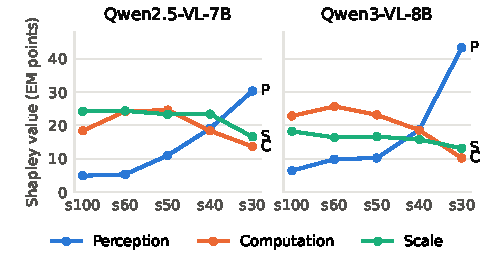
\includegraphics[width=\columnwidth]{fig/attr}
\caption{Shapley values by image quality. P, C and S mark the end of each series.}
\label{fig:attr}
\end{figure}

\section{Reading Experiments}
\label{sec:method}

\paragraph{Cells.} The planned set has 500 target cells, one per document, disjoint from the attribution set: numeric, at least three digits, unique on the page, with row and column labels found through OCR. Models are the two above plus InternVL3-8B \citep{zhu2025internvl3} with tiling enabled, since the checkpoint default squeezes a page into one 448\,px tile. Decoding is greedy. Prompts name the row and column labels and ask for the number. \textbf{The run stopped at \val{seven.n}, \val{three.n} and \val{intern.n} complete cells}; the cells are taken in a fixed shuffled order, and the stop did not depend on results.

\paragraph{Digit edits.} We delete the number in pixels using the modal background colour and redraw it in a matched font, in three versions: unchanged (null), one interior digit replaced (counterfactual, cf), and, as a placebo, a digit value never drawn. $T$ is the rate of outputting the drawn number, $O$ the deleted original, $A$ the placebo.

\paragraph{Factorial.} All four conditions downsample the page and enlarge it back to its original size with bicubic interpolation, which equalizes image tokens. \emph{Base} is that canvas. $G$ pastes the original pixels back over every numeric OCR word on the page, excluding year-like words unless they are the target, so sharpness does not reveal the target and labels stay blurred. $L$ draws a red box around the target and tells the model so. We report two-player Shapley values $\phi_L,\phi_G$ on $T$ and their interaction. \emph{Real} is the actual downsampled page, with fewer tokens (on a 1240$\times$1605 page, 7B receives about 285 image tokens at s30 and 2,508 at original size).

\paragraph{Confidence and refusal.} We compare mean-token log-probability with a stated 0--100 confidence, and offer an UNREADABLE option under two wordings. Blank pages provide a floor.

\paragraph{Criteria.} Table~\ref{tab:verdicts} applies the locked criteria. D1 requires both $\phi_L$ and $\phi_G$ to have intervals above zero at one level. D2 asks whether $O-A$ is at least 3 points with an interval above zero. D3 asks whether copying and writing an expression differ by at least 5 points. D4a requires log-probability AUROC of at least 0.75 at s40 and s30, above that of glyph height, with discordant within-cell pairs above 50\%.\footnote{The protocol does not state the levels for the discordant-pair part. We apply the stricter reading, both levels.} D4b requires a refusal gap of at least 20 points at s30. D4c requires log-probability AUROC to exceed that of stated confidence.

\begin{table}[t]
\centering\small
\begin{tabular}{@{}lccc@{}}
\toprule
Criterion & 7B & Qwen3 & InternVL \\
\midrule
Valid & yes & yes & yes \\
D1 separable & no & no & no \\
D2 context pull & negligible & negligible & negligible \\
D3 task dependence & open & open & yes \\
D4a hidden signal & yes & no & no \\
D4b verbal refusal & no & no & no \\
D4c signal--speech gap & yes & yes & yes \\
\bottomrule
\end{tabular}

\caption{Locked criteria on the incomplete sample. All are provisional. For D1, the entry lists qualifying levels.}
\label{tab:verdicts}
\end{table}

\section{Results}

\paragraph{Validity.} At s100, the null edit shifts $T$ by \val{seven.null}, \val{three.null} and \val{intern.null} points; $T$(cf) is \val{seven.cf}, \val{three.cf} and \val{intern.cf}; and a box alone directs copying to a decoy cell at \val{seven.box}, \val{three.box} and \val{intern.box}\%. All three models pass, so the edits and the box function as intended.

\paragraph{Models read what is drawn.} $O-A$ at s30 is \val{seven.s30.pull} on 7B and \val{three.s30.pull} on Qwen3, and D2 classes the context pull as negligible on all three (Table~\ref{tab:cf}). InternVL produced no original-digit outputs in this sample, so its interval is degenerate. The task effect is less uniform. It is inconclusive on the Qwen models and present on InternVL, where copying beats writing an expression by \val{intern.s50.task} points at s50. That criterion compares output formats and does not establish a difference in perception.

\begin{table}[t]
\centering\small
\resizebox{\columnwidth}{!}{\begin{tabular}{@{}llrrr@{}}
\toprule
Model & Lvl & $T$(cf) & $O-A$ & $T$(copy)$-T$(expr) \\
\midrule
7B & s50 & 70.6 & +0.9 & $+1.4$ {\scriptsize[-2.3, +5.5]} \\
 & s40 & 49.5 & +0.9 & $+4.6$ {\scriptsize[+0.0, +9.6]} \\
 & s30 & 26.1 & +0.9 & $+3.7$ {\scriptsize[+0.0, +7.8]} \\
Qwen3 & s50 & 73.5 & +1.2 & $+1.2$ {\scriptsize[-2.3, +4.2]} \\
 & s40 & 56.2 & +0.0 & $-0.8$ {\scriptsize[-4.2, +2.7]} \\
 & s30 & 9.2 & +0.4 & $+1.5$ {\scriptsize[-1.5, +5.0]} \\
Intern & s50 & 80.3 & +0.0 & $+7.1$ {\scriptsize[+1.6, +13.4]} \\
 & s40 & 78.7 & +0.0 & $+7.9$ {\scriptsize[+0.8, +15.7]} \\
 & s30 & 59.1 & +0.0 & $+3.1$ {\scriptsize[-3.9, +10.2]} \\
\bottomrule
\end{tabular}
}
\caption{Digit edits. $T-$ columns are point differences with 95\% intervals.}
\label{tab:cf}
\end{table}

\paragraph{The factorial.} \textbf{The locked separability criterion D1 was not met at any level on any model}, so our preregistered stop rule for this part is triggered on the present sample. It was also unstable across looks: Qwen3 and InternVL each met it at s50 at a smaller interim sample, and $\phi_L$ at s40 on 7B has a lower bound at zero. The pattern is in Table~\ref{tab:factorial}. What follows is exploratory.

$\phi_L$ is largest at s50 (\val{seven.s50.phiL} on 7B, \val{three.s50.phiL} on Qwen3), where restored pixels add almost nothing. $\phi_G$ is largest at s30 (\val{seven.s30.phiG}, \val{three.s30.phiG}, \val{intern.s30.phiG}), where $\phi_L$ cannot be told from zero. This crossover suggests that position limits reading at mild degradation and legibility at severe degradation. We chose this reading after seeing the data.

The interaction at s30 is large and positive (\val{seven.s30.inter}, \val{three.s30.inter}, \val{intern.s30.inter}). On blurred pixels the box does not help at s30 and can harm: \val{seven.s30.boxBlur}, \val{three.s30.boxBlur}, \val{intern.s30.boxBlur}. On restored pixels it helps: \val{seven.s30.boxSharp}, \val{three.s30.boxSharp}, \val{intern.s30.boxSharp}. The harm may be an artifact, since a box can cover small blurred glyphs, and so $\phi_L$ may understate the value of position. Published box nulls \citep{shi2026readaloud,xia2026foundnotread} come from compressed pages and many-page contexts; ours concern a single table and may differ for that reason.

\begin{table}[t]
\centering\small\setlength{\tabcolsep}{3.5pt}
\resizebox{\columnwidth}{!}{\begin{tabular}{@{}llrrrrrr@{}}
\toprule
Model & Lvl & Real & Base & $L$ & $G$ & $LG$ & $\phi_L$ / $\phi_G$ \\
\midrule
7B & s50 & 80.7 & 86.7 & 90.4 & 85.3 & 93.1 & +5.7* / +0.7 \\
 & s40 & 61.0 & 84.9 & 84.4 & 84.4 & 94.0 & +4.6 / +4.6* \\
 & s30 & 38.5 & 68.8 & 65.1 & 85.3 & 92.2 & +1.6 / +21.8* \\
Qwen3 & s50 & 78.1 & 86.5 & 93.8 & 87.3 & 95.4 & +7.7* / +1.2 \\
 & s40 & 60.4 & 85.8 & 85.8 & 87.3 & 95.0 & +3.8 / +5.4* \\
 & s30 & 16.2 & 79.2 & 62.3 & 85.4 & 94.2 & -4.0 / +19.0* \\
Intern & s50 & 81.9 & 82.7 & 84.3 & 81.1 & 90.6 & +5.5 / +2.4* \\
 & s40 & 80.3 & 80.3 & 76.4 & 79.5 & 90.6 & +3.5 / +6.7* \\
 & s30 & 62.2 & 63.0 & 44.9 & 76.4 & 88.2 & -3.1 / +28.3* \\
\bottomrule
\end{tabular}
}
\caption{Percentage of cells read correctly. Real has fewer tokens on Qwen models; the other columns share a canvas. * marks intervals excluding zero.}
\label{tab:factorial}
\end{table}

\begin{figure}[t]
\centering
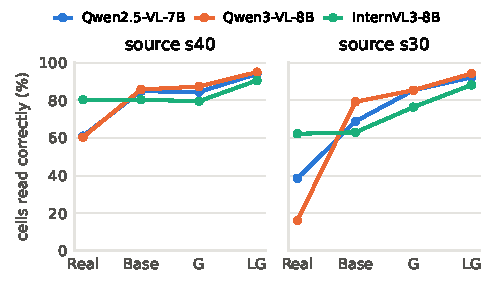
\includegraphics[width=\columnwidth]{fig/ladder}
\caption{Reading rate from the real downsampled page through enlargement (Base), restored pixels (G), and box (LG).}
\label{fig:ladder}
\end{figure}

\paragraph{Enlargement.} Enlarging adds no information, yet Base exceeds Real by \val{seven.s30.upscale} points on 7B and \val{three.s30.upscale} on Qwen3 at s30 (Figure~\ref{fig:ladder}). On InternVL it adds \val{intern.s30.upscale}, as expected when both inputs become the same tile grid. This replicates on table cells what \citet{shi2026readaloud} shows on prose. Reporting this difference was planned, but the inference is post hoc, since we noticed it at an interim look. A locked follow-up on fresh cells (\texttt{protocol\_token}) was stopped after too few cells to analyse, so its criteria remain untested.

For Qwen3 at s30, the steps are \val{three.s30.orig} (Real), \val{three.s30.base} (Base), \val{three.s30.G} ($G$), \val{three.s30.LG} ($LG$). Most of the attribution curve's perception loss at s30 on this model may therefore reflect the input size rather than destroyed information. This inference crosses experiments, one on question answering and one on copying, and we did not test it directly.

\paragraph{Confidence.} Stated confidence carries almost no information (AUROC \val{seven.s30.auc}, \val{three.s30.auc}, \val{intern.s30.auc} at s30), and D4c holds on all three (Table~\ref{tab:meta}). Excluding InternVL's few out-of-scale outputs leaves its AUROC at \val{intern.s30.aucin}. Log-probability reaches \val{seven.s30.au}, \val{three.s30.au} and \val{intern.s30.au}. The stronger D4a passes only on 7B; Qwen3's discordant-pair interval at s30 includes 50\% (\val{three.s30.disc}), and InternVL at s40 rests on few cells. So log-probability separates correct from incorrect readings across cells, while within-cell evidence is firm only on 7B.

\paragraph{Refusal.} D4b fails on all three models: the \texttt{UNREADABLE} gap at s30 is \val{seven.s30.refgap}, \val{three.s30.refgap} and \val{intern.s30.refgap} under the stronger wording. Qwen3 falls just short of the 20-point threshold. Silence is not absolute either. All three models refuse 100\% of blank pages under that wording, and refuse \val{seven.s30.refrate}, \val{three.s30.refrate} and \val{intern.s30.refrate}\% at s30. Under the plain prompt, they output a number on \val{seven.blank}, \val{three.blank} and \val{intern.blank}\% of blank pages.

\begin{table}[t]
\centering\small\setlength{\tabcolsep}{3.5pt}
\resizebox{\columnwidth}{!}{\begin{tabular}{@{}llrrrrr@{}}
\toprule
Model & Lvl & Correct & AUROC$_{lp}$ & AUROC$_{conf}$ & Refusal & Refusal gap \\
\midrule
7B & s40 & 61.0 & 0.82 & 0.50 & 6.0 & +5.7 \\
 & s30 & 38.5 & 0.87 & 0.51 & 6.9 & +11.2 \\
Qwen3 & s40 & 60.4 & 0.75 & 0.51 & 8.5 & +10.1 \\
 & s30 & 16.2 & 0.85 & 0.47 & 16.5 & +19.7 \\
Intern & s40 & 80.3 & 0.76 & 0.45 & 9.4 & +23.1 \\
 & s30 & 62.2 & 0.79 & 0.47 & 12.6 & +13.2 \\
\bottomrule
\end{tabular}
}
\caption{Log-probability vs stated confidence, and refusal under the stronger wording. Gap: P(refuse\,$|$\,wrong)$-$P(refuse\,$|$\,right), points.}
\label{tab:meta}
\end{table}

\section{Limitations}
\label{sec:limits}

\paragraph{Incomplete sample.} We committed to conclude only from 500 cells and did not reach them: 44\%, 52\% and 25\% of the plan. InternVL's estimates are especially wide. Two interim looks occurred, one requested and one during tooling tests, and verdicts changed between them. D1 and D4a in particular sit near boundaries. No threshold or scoring rule changed after looking. There is no multiplicity correction.

\paragraph{Unconfirmed explanation.} Enlargement changes token count and glyph size per patch together, and interpolation may matter; our follow-up was to examine this and did not complete. We cannot claim a token-budget mechanism.

\paragraph{Unexplained disagreement.} \citet{shi2026readaloud} reports a read-use gap on Qwen3-VL-8B even with gold evidence alone, whereas we find little task effect on Qwen models. Multi-hop prose answering and copying one cell differ, but we did not test whether that accounts for it.

\paragraph{Stimuli and scope.} Downsampling is simulated and the box and pasted sharpness are artificial cues. Edits use substitute fonts. Our sets require facts matching OCR, and all data come from one domain. Attribution's $P$ player is coarse. We tested three open models, and InternVL3-8B differs from the InternVL3.5 of prior work.

\section{Conclusion}

Perception's share of question-answering loss grows sharply as financial pages lose resolution, and models then read what is drawn rather than what context suggests. Our provisional data suggest this perception loss is not one thing: some may come from input size, some from destroyed glyphs, and some from position, with position and legibility trading places as degradation worsens. The preregistered separability test did not pass, so this structure is a hypothesis for the completed run, not a finding. Completing the planned sample and the token follow-up are the next steps, and a second dataset with real captures is needed before generalizing.

\bibliography{refs}

\end{document}
